\subsection{实验目的}
掌握一些基本的图像融合方法,包括基于像素灰度值的简单图像融合算法,以及彩色图像的分解于合成。完成遥感图像的图像融合。
\subsection{实验原理}
\subsubsection{图像融合的概念}
综合和提取两个或多个圆的图像信息,获得对同一场景或者目标更为准确、全面、可靠的图像,使之更适合人眼感知或计算机后续处理。
\begin{figure}[H]
	\centering
	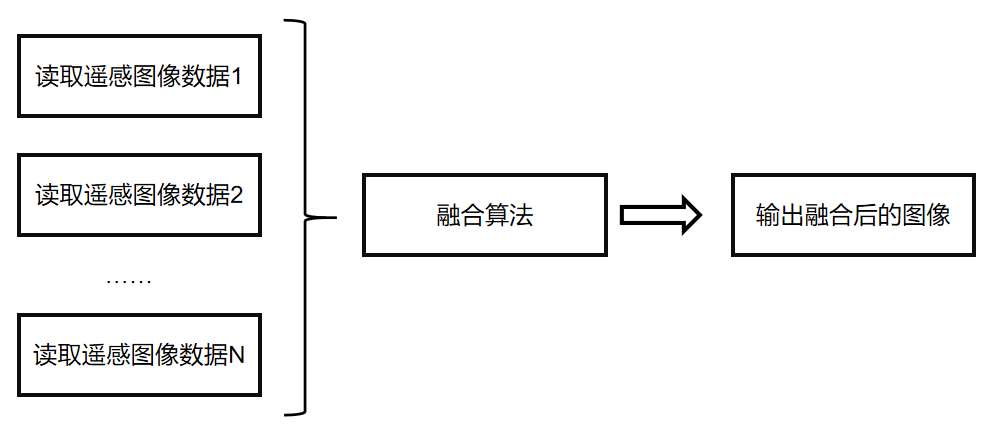
\includegraphics[width=0.7\linewidth]{figure/fusion_flowchart.png}
	\caption{图像融合算法流程图}
	\label{fig:fusion_flowchart}
\end{figure}
\subsubsection{简单的图像融合算法}
\begin{description}
	\item[像素灰度值平均或加权平均法]
	\[ I(x, y)=\frac{\sum_{n=1}^{N}W^n(x, y)I^n(x, y)}{\sum_{n=1}^{N}W^n(x, y)} \]
	\[ W^n(x, y)=\frac{1}{N} \]
	\item[像素灰度值选大法] 
	\[ I(x, y)=\max_n\{I^n(x, y),\quad n=1,2,\dots N\} \]
	\item[像素灰度值选小法] 
	\[ I(x, y)=\min_n\{I^n(x, y),\quad 1,2,\dots N\} \]
\end{description}
\subsubsection{彩色图像的分解与合成}
\begin{description}
	\item[能量图像] 
	\[ I=Ir+Ig+Ib \]
	\item[变换后的彩色图像合成]
	蓝色分量:加高斯噪声污染
	
	绿色分量:进行对数变换
	
	红色分量:进行图像反转
	
	重新合成彩色图像
\end{description}
\subsubsection{彩色图像合成}
通过图像变换与融合突出图像中感兴趣的目标。
\subsubsection{通过图像融合得到变化检测差异图}
\begin{description}
	\item[差异图像] 
	\[ I1=1-\min \left( \frac{\mu_1}{\mu_2},\frac{\mu_2}{\mu_1} \right)  \]
	\[ I2= \left| \log\frac{X_2}{X_1} \right| = \left| \log X_2 - \log X_1 \right|  \]
	\item[图像融合]
	两个差异图的低频成分平均融合,高频成分取小融合。
\end{description}
\subsection{实验流程}
\subsection{实验程序}
\subsection{实验结果和分析}